\chapter{Practice set solutions}
\begin{abox}
	Problem Set -3
\end{abox}
\begin{enumerate}[label=\color{ocre}\textbf{\arabic*.}]
	\item  Let $p_{n}(x)$ (where $n=0,1,2, \ldots \ldots$ ) be a polynomial of degree $n$ with real coefficients, defined in the interval $2 \leq n \leq 4$. If $\int_{2}^{4} p_{n}(x) p_{m}(x) d x=\delta_{n m}$, then
	{\exyear{NET/JRF(JUNE-2011)}}
	\begin{tasks}(2)
		\task[\textbf{A.}] $p_{0}(x)=\frac{1}{\sqrt{2}}$ and $p_{1}(x)=\sqrt{\frac{3}{2}}(-3-x)$
		\task[\textbf{B.}]  $p_{0}(x)=\frac{1}{\sqrt{2}}$ and $p_{1}(x)=\sqrt{3}(3+x)$
		\task[\textbf{C.}] $p_{0}(x)=\frac{1}{2}$ and $p_{1}(x)=\sqrt{\frac{3}{2}}(3-x)$
		\task[\textbf{D.}] $p_{0}(x)=\frac{1}{\sqrt{2}}$ and $p_{1}(x)=\sqrt{\frac{3}{2}}(3-x)$
	\end{tasks}
	\begin{answer}
		For $n$ not equal to $m$ kroneker delta become zero. One positive and one negative term can make integral zero. So answer may be (C) or (D). Now take $n=m=0$ so $p_{0}(x)=\frac{1}{\sqrt{2}}$ and then integrate. (D) is correct option because it satisfies the equation Check by integration and by orthogonal property of Legendre polynomial also.\\\\
		So the correct answer is \textbf{Option (D)}
	\end{answer}
	\item  The generating function $F(x, t)=\sum_{n=0}^{\infty} P_{n}(x) t^{n}$ for the Legendre polynomials $P_{n}(x)$ is $F(x, t)=\left(1-2 x t+t^{2}\right)^{-1 / 2}$. The value of $P_{3}(-1)$ is
	{\exyear{NET/JRF(DEC-2011)}}
	\begin{tasks}(4)
		\task[\textbf{A.}] $5 / 2$
		\task[\textbf{B.}] $3 / 2$
		\task[\textbf{C.}] $+1$
		\task[\textbf{D.}] $-1$
	\end{tasks}
	\begin{answer}
		\begin{align*}
		P_{3}&=\frac{1}{2}\left(5 x^{3}-3 x\right) \Rightarrow P_{3}(-1)\\&=\frac{1}{2}\left(5(-1)^{3}-3(-1)\right)=\frac{1}{2}[-5+3]=-1
		\end{align*}
		So the correct answer is \textbf{Option (D)}
	\end{answer}
	\item  The graph of the function $f(x)$ shown below is best described by
	{\exyear{NET/JRF(DEC-2012)}}
	\begin{figure}[H]
		\centering
		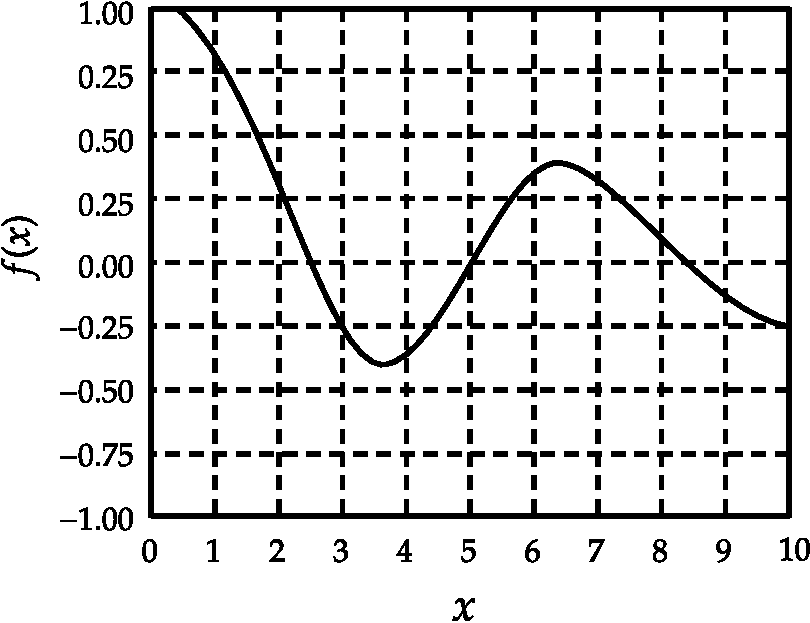
\includegraphics[height=6cm,width=8cm]{diagram-20211005(12)-crop}
	\end{figure}
	\begin{tasks}(2)
		\task[\textbf{A.}]  The Bessel function $J_{0}(x)$
		\task[\textbf{B.}] $\cos x$
		\task[\textbf{C.}] $e^{-x} \cos x$
		\task[\textbf{D.}] $\frac{1}{x} \cos x$
	\end{tasks}
	\begin{answer}
		So the correct answer is \textbf{Option (A)}
	\end{answer}
	\item Given that $\sum_{n=0}^{\infty} H_{n}(x) \frac{t^{n}}{n !}=e^{-t^{2}+2 t x}$ the value of $H_{4}(0)$ is
	{\exyear{NET/JRF(JUNE-2013)}}
	\begin{tasks}(4)
		\task[\textbf{A.}] 12
		\task[\textbf{B.}] 6
		\task[\textbf{C.}] 24
		\task[\textbf{D.}] $-6$
	\end{tasks}
	\begin{answer}
		\begin{align*}
		\sum_{n=0}^{\infty} H_{n}(x) \frac{t^{n}}{n !}&=e^{-t^{2}+2 x} \Rightarrow \sum_{n=0}^{\infty} H_{n}(0) \frac{t^{n}}{n !}\\&=e^{-t^{2}}=1-t^{2}+\frac{t^{4}}{2 !}-\frac{t^{6}}{3 !}\\
		\Rightarrow \frac{H_{4}(0)}{4 !} t^{4}&=\frac{t^{4}}{2 !} \Rightarrow H_{4}(0)=\frac{4 !}{2 !}=12
		\end{align*}
		So the correct answer is \textbf{Option (A)}
	\end{answer}
	\item   Given $\sum_{n=0}^{\infty} P_{n}(x) t^{n}=\left(1-2 x t+t^{2}\right)^{-1 / 2}$, for $|t|<1$, the value of $P_{5}(-1)$ is
	{\exyear{NET/JRF(JUNE-2014)}}
	\begin{tasks}(4)
		\task[\textbf{A.}] $0.26$
		\task[\textbf{B.}] 1
		\task[\textbf{C.}] $0.5$
		\task[\textbf{D.}] $-1$
	\end{tasks}
	\begin{answer}
		\begin{align*}
		P_{n}(-1)&=-1\text{ if }n\text{ is odd }\Rightarrow P_{5}(-1)=-1
		\end{align*}
		So the correct answer is \textbf{Option (D)}
	\end{answer}
	\item The function $f(x)=\sum_{n=0}^{\infty} \frac{(-1)^{n}}{n !(n+1) !}\left(\frac{x}{2}\right)^{2 n+1}$, satisfies the differential equation
	{\exyear{NET/JRF(DEC-2014)}}
	\begin{tasks}(2)
		\task[\textbf{A.}]  $x^{2} \frac{d^{2} f}{d x^{2}}+x \frac{d f}{d x}+\left(x^{2}+1\right) f=0$
		\task[\textbf{B.}]  $x^{2} \frac{d^{2} f}{d x^{2}}+2 x \frac{d f}{d x}+\left(x^{2}-1\right) f=0$
		\task[\textbf{C.}] $x^{2} \frac{d^{2} f}{d x^{2}}+x \frac{d f}{d x}+\left(x^{2}-1\right) f=0$
		\task[\textbf{D.}] $x^{2} \frac{d^{2} f}{d x^{2}}-x \frac{d f}{d x}+\left(x^{2}-1\right) f=0$
	\end{tasks}
	\begin{answer}
		\begin{align*}
		\intertext{ $f(x)=\sum_{n=0}^{\infty} \frac{(-1)^{n}}{n !(n+1) !}\left(\frac{x}{2}\right)^{2 n+1}$ is generating function (Bessel Function of first kind) which satisfies the differential equation $x^{2} \frac{d^{2} f}{d x^{2}}+x \frac{d f}{d x}+\left(x^{2}-n^{2}\right) f=0$, put $n=1$.}
		\end{align*}
		So the correct answer is \textbf{Option (C)}
	\end{answer}
	\item
	The Hermite polynomial $H_{n}(x)$, satisfies the differential equation
	$$
	\frac{d^{2} H_{n}}{d x^{2}}-2 x \frac{d H_{n}}{d x}+2 n H_{n}(x)=0
	$$
	The corresponding generating function $G(t, x)=\sum_{n=0}^{\infty} \frac{1}{n !} H_{n}(x) t^{n}$, satisfies the equation
	{\exyear{NET/JRF(DEC-2015)}}
	\begin{tasks}(2)
		\task[\textbf{A.}] $\frac{\partial^{2} G}{\partial x^{2}}-2 x \frac{\partial G}{\partial x}+2 t \frac{\partial G}{\partial t}=0$
		\task[\textbf{B.}] $\frac{\partial^{2} G}{\partial x^{2}}-2 x \frac{\partial G}{\partial x}-2 t^{2} \frac{\partial G}{\partial t}=0$
		\task[\textbf{C.}] $\frac{\partial^{2} G}{\partial x^{2}}-2 x \frac{\partial G}{\partial x}+2 \frac{\partial G}{\partial t}=0$
		\task[\textbf{D.}]  $\frac{\partial^{2} G}{\partial x^{2}}-2 x \frac{\partial G}{\partial x}+2 \frac{\partial^{2} G}{\partial x \partial t}=0$
	\end{tasks}
	\begin{answer}
		\begin{align*}
		G&=\frac{1}{n !} H_{n}(x) t^{n}, G^{\prime}=\frac{1}{n !} H_{n}^{\prime}(x) t^{n}, G^{\prime \prime}=\frac{1}{n !} H_{n}^{\prime \prime}(x) t^{n}\\
		\frac{\partial G}{\partial t}&=\frac{1}{n !} H_{n}(x) n t^{n-1}
		\intertext{Let's check the options one by one}
		\frac{\partial G}{\partial x^{2}}&-2 x \frac{\partial G}{\partial x}+2 t \frac{\partial G}{\partial t}=0\\
		\frac{1}{n !} H_{n}^{\prime \prime}(x) t^{n}&-2 x \frac{1}{n !} H_{n}^{\prime}(x) t^{n}+2 t \frac{1}{n !} H_{n}(x) n t^{n-1}\\
		H_{n}^{\prime \prime}(x)-2 x H_{n}^{\prime}(x)+2 x H_{n}(x)&=0,\text{ which is Hermite Differential Equation.}
		\end{align*}
		So the correct answer is \textbf{Option (A)}
	\end{answer}
	\item A stable asymptotic solution of the equation $x_{n+1}=1+\frac{3}{1+x_{n}}$ is $x=2$. If we take $x_{n}=2+\epsilon_{n}$ and $x_{n+1}=2+\epsilon_{n+1}$, where $\epsilon_{n}$ and $\epsilon_{n+1}$ are both small, the ratio $\frac{\epsilon_{n+1}}{\epsilon_{n}}$ is approximately
	{\exyear{NET/JRF(DEC-2016)}}
	\begin{tasks}(4)
		\task[\textbf{A.}] $-\frac{1}{2}$
		\task[\textbf{B.}] $-\frac{1}{4}$
		\task[\textbf{C.}]  $-\frac{1}{3}$
		\task[\textbf{D.}] $-\frac{2}{3}$
	\end{tasks}
	\begin{answer}
		So the correct answer is \textbf{Option (C)}
	\end{answer}
	\item  The Green's function satisfying
	$$
	\frac{d^{2}}{d x^{2}} g\left(x, x_{0}\right)=\delta\left(x-x_{0}\right)
	$$
	with the boundary conditions $g\left(-L, x_{0}\right)=0=g\left(L, x_{0}\right)$, is
	{\exyear{NET/JRF(JUNE-2017)}}
	\begin{tasks}(1)
		\task[\textbf{A.}] $\left\{\begin{array}{ll}\frac{1}{2 L}\left(x_{0}-L\right)(x+L), & -L \leq x<x_{0} \\ \frac{1}{2 L}\left(x_{0}+L\right)(x-L), & x_{0} \leq x \leq L\end{array}\right.$
		\task[\textbf{B.}]  $\left\{\begin{array}{ll}\frac{1}{2 L}\left(x_{0}+L\right)(x+L), & -L \leq x<x_{0} \\ \frac{1}{2 L}\left(x_{0}-L\right)(x-L), & x_{0} \leq x \leq L\end{array}\right.$
		\task[\textbf{C.}] $\left\{\begin{array}{ll}\frac{1}{2 L}\left(L-x_{0}\right)(x+L), & -L \leq x<x_{0} \\ \frac{1}{2 L}\left(x_{0}+L\right)(L-x), & x_{0} \leq x \leq L\end{array}\right.$
		\task[\textbf{D.}] $\frac{1}{2 L}(x-L)(x+L), \quad-L \leq x \leq L$
	\end{tasks}
	\begin{answer}
		\begin{align*}
		\frac{d^{2}}{d x^{2}} g\left(x, x_{0}\right)&=\delta\left(x-x_{0}\right)
		\intertext{word or phrase}
		g\left(-L, x_{0}\right)&=0=g\left(L, x_{0}\right)
		\intertext{The homogeneous equation for Green's function is}
		\frac{d^{2}}{d x^{2}} g\left(x, x_{0}\right)&=0
		\intertext{Solution of above equation is}
		g\left(x, x_{0}\right)&=\left\{\begin{array}{ll}A x+B, & x<x_{0} \\ C x+D, & x>x_{0}\end{array}\right.
		\intertext{Applying boundary condition}
		g\left(-L, x_{0}\right)&=0 \Rightarrow-A L+B=0 \Rightarrow A L=B\\
		g\left(L, x_{0}\right)&=0 \Rightarrow C L+D=0 \Rightarrow-C L=D\\
		\text{Hence, }g\left(x, x_{0}\right)&=\left\{\begin{array}{ll}A(x+L), & x<x_{0} \\ C(x-L), & x>x_{0}\end{array}\right.
		\intertext{From continuity of Green's function at $x=x_{0}$ we have}
		A\left(x_{0}+L\right)&=C\left(x_{0}-L\right)\\
		A&=C\left(\frac{x_{0}-L}{x_{0}+L}\right)
		\intertext{From discontinuity of derivative of Green's function $\frac{\partial g}{\partial x}$ at $x=x_{0}$}
		\intertext{We have}
		\left|\frac{\partial g}{\partial x}\right|_{x=x_{0}^{+}}-\left.\frac{\partial g}{\partial x}\right|_{x=x_{0}^{-}}&=1\\
		\left|\frac{\partial g}{\partial x}\right|_{x=x_{0}^{+}}=C,\left.\frac{\partial g}{\partial x}\right|_{x=x_{0}^{-}}&=A\\
		\therefore C-A&=1 \Rightarrow C=A+1
		\intertext{Thus, the required solution of Green's function is given by}
		g\left(x, x_{0}\right)&=\left\{\begin{array}{ll}\frac{\left(x_{0}-L\right)(x+L)}{2 L}, & x<x_{0} \\ \frac{\left(x_{0}+L\right)(x-L)}{2 L}, & x>x_{0}\end{array}\right.
		\end{align*}
		So the correct answer is \textbf{Option (A)}
	\end{answer}
	\item  The generating function $G(t, x)$ for the Legendre polynomials $P_{n}(t)$ is
	$$
	G(t, x)=\frac{1}{\sqrt{1-2 x t+x^{2}}}=\sum_{n=0}^{\infty} x^{n} P_{n}(t), \text { for }|x|<1
	$$
	If the function $f(x)$ is defined by the integral equation $\int_{0}^{x} f\left(x^{\prime}\right) d x^{\prime}=x G(1, x)$, it can be expressed as
	{\exyear{NET/JRF(DEC-2017)}}
	\begin{tasks}(2)
		\task[\textbf{A.}] $\sum_{n, m=0}^{\infty} x^{n+m} P_{n}(1) P_{m}\left(\frac{1}{2}\right)$
		\task[\textbf{B.}] $\sum_{n, m=0}^{\infty} x^{n+m} P_{n}(1) P_{m}(1)$
		\task[\textbf{C.}] $\sum_{n, m=0}^{\infty} x^{n-m} P_{n}(1) P_{m}(1)$
		\task[\textbf{D.}] $\sum_{n, m=0}^{\infty} x^{n-m} P_{n}(0) P_{m}(1)$
	\end{tasks}
	\begin{answer}
		\begin{align*}
		G(t, x)&=\frac{1}{\sqrt{1-2 x t+x^{2}}}=\sum_{n=0}^{\infty} x^{n} P_{n}(t)\text{ for }|x|<1\\
		G(1, x)&=\frac{1}{\sqrt{1-2 x+x^{2}}}=\sum_{n=0}^{\infty} x^{n} P_{n}(1)\\
		&=\frac{1}{\sqrt{(1-x)^{2}}}=\sum_{n=0}^{\infty} x^{n} P_{n}(1)\\&=\frac{1}{1-x}\text{ Since } |x|<1\\
		\text{Now, }x \cdot \frac{1}{1-x}&=\int_{0}^{x} f\left(x^{\prime}\right) d x^{\prime}
		\intertext{Differentiating both sides,}
		f(x)&=\frac{d}{d x} \frac{x}{1-x}=\frac{1}{(1-x)^{2}}
		\end{align*}
		So the correct answer is \textbf{Option (B)}
	\end{answer}
	\item In the function $P_{n}(x) e^{-x^{2}}$ of a real variable $x, P_{n}(x)$ is polynomial of degree $n$. The maximum number of extrema that this function can have is
	{\exyear{NET/JRF(JUNE-2018)}}
	\begin{tasks}(4)
		\task[\textbf{A.}] $n+2$
		\task[\textbf{B.}]  $n-1$
		\task[\textbf{C.}] $n+1$
		\task[\textbf{D.}] $n$
	\end{tasks}
	\begin{answer}
		\begin{align*}
		y&=P_{n}(x) e^{-x^{2}} \Rightarrow P_{n}^{\prime}(x) e^{-x^{2}}+P_{n}(x) e^{-x^{2}}(-2 x)\\
		&=0 \Rightarrow P_{n}^{\prime}(x)-2 x P_{n}(x)=0\\
		P_{0}(x)=1, P_{1}(x)&=2 \Rightarrow P_{0}^{\prime}(x)-2 x P_{0}(x)\\&=0 \Rightarrow 0-2 x .1=0\\
		x&=0,1\text{ extrema}\\
		P_{1}^{\prime}(x)-2 x P_{1}(x)&=0\\
		1-2 x \cdot x&=0 \Rightarrow x=\pm \frac{1}{\sqrt{2}}\text{ i.e., 2 extrema.}\\
		\text{Thus in general there are }&(n+1)\text{ extrema.}
		\end{align*}
		So the correct answer is \textbf{Option (C)}
	\end{answer}
	\item  The Green's function $G\left(x, x^{\prime}\right)$ for the equation $\frac{d^{2} y(x)}{d x^{2}}+y(x)=f(x)$, with the boundary values $y(0)=y\left(\frac{\pi}{2}\right)=0$, is
	{\exyear{NET/JRF(JUNE-2018)}}
	\begin{tasks}(1)
		\task[\textbf{A.}] $G\left(x, x^{\prime}\right)=\left\{\begin{array}{ll}x\left(x^{\prime}-\frac{\pi}{2}\right), & 0<x<x^{\prime}<\frac{\pi}{2} \\ \left(x-\frac{\pi}{2}\right) x^{\prime}, & 0<x^{\prime}<x<\frac{\pi}{2}\end{array}\right.$
		\task[\textbf{B.}] $G\left(x, x^{\prime}\right)=\left\{\begin{array}{ll}-\cos x^{\prime} \sin x, & 0<x<x^{\prime}<\frac{\pi}{2} \\ -\sin x^{\prime} \cos x, & 0<x^{\prime}<x<\frac{\pi}{2}\end{array}\right.$
		\task[\textbf{C.}] $G\left(x, x^{\prime}\right)=\left\{\begin{array}{ll}\cos x^{\prime} \sin x, & 0<x<x^{\prime}<\frac{\pi}{2} \\ \sin x^{\prime} \cos x, & 0<x^{\prime}<x<\frac{\pi}{2}\end{array}\right.$
		\task[\textbf{D.}] $G\left(x, x^{\prime}\right)=\left\{\begin{array}{ll}x\left(\frac{\pi}{2}-x^{\prime}\right), & 0<x<x^{\prime}<\frac{\pi}{2} \\ x^{\prime}\left(\frac{\pi}{2}-x\right), & 0<x^{\prime}<x<\frac{\pi}{2}\end{array}\right.$
	\end{tasks}
	\begin{answer}
		\begin{align*}
		\frac{d^{2} y}{d x^{2}}+y&=0 \Rightarrow m^{2}+1=0 \Rightarrow m=0 \pm i\\
		y_{1}(x)&=\sin x(a t), y_{1}^{\prime}(x)=\cos x\\
		y_{2}(x)&=\cos x \quad\left(a t \frac{\pi}{2}\right), y_{2}^{\prime}(x)=-\sin x\\
		A&=\left\{P\left(x^{\prime}\right)\left[y_{2}^{\prime}\left(x^{\prime}\right) y_{1}\left(x_{1}^{\prime}\right)-y_{1}^{\prime}\left(x^{\prime}\right)\right] y_{2}\left(x^{\prime}\right)\right\}\\
		\Rightarrow A&=\left\{-\sin x^{\prime} \sin x^{\prime}-\cos ^{\prime} \cos x^{\prime}\right\} \\ \because P(x)&=1 \Rightarrow A=-1\\
		\text{Thus }G\left(x, x^{\prime}\right)&=\left\{\begin{array}{ll}A y_{1}(x) y_{2}\left(x^{\prime}\right), & x<x^{\prime} \\ A y_{2}(x) y_{1}(x), & x>x^{\prime}\end{array}=\left\{\begin{array}{ll}-\sin x \cos x^{\prime}, & 0<x<x^{\prime}<\frac{\pi}{2} \\ -\cos x \sin x^{\prime}, & 0<x^{\prime}<x<\frac{\pi}{2}\end{array}\right.\right.
		\end{align*}
		So the correct answer is \textbf{Option (B)}
	\end{answer}
	\item The polynomial $f(x)=1+5 x+3 x^{2}$ is written as linear combination of the Legendre polynomials
	$\left(P_{0}(x)=1, P_{1}(x), P_{2}(x)=\frac{1}{2}\left(3 x^{2}-1\right)\right)$ as $f(x)=\sum_{n} c_{n} P_{n}(x)$. The value of $c_{0}$ is
	{\exyear{NET/JRF(DEC-2018)}}
	\begin{tasks}(4)
		\task[\textbf{A.}] $\frac{1}{4}$
		\task[\textbf{B.}] $\frac{1}{2}$
		\task[\textbf{C.}]  2
		\task[\textbf{D.}]  4
	\end{tasks}
	\begin{answer}
		\begin{align*}
		f(x)&=1+5 x+3 x^{2}\\
		1&=P_{0}(x) \quad x=P_{1}(x)\\
		x^{2}&=\frac{1}{3}\left(2 P_{2}(x)+1\right)\\
		f(x)&=P_{0}(x)+5 P_{1}(x)+2 P_{2}(x)+P_{0}(x)\\
		&=2 P_{0}(x)+5 P_{1}(x)+2 P_{2}(x)\\
		&=c_{0} P_{0}(x)+c_{1} P_{1}(x)+c_{2} P_{2}(x) c_{0}=2
		\end{align*}
		So the correct answer is \textbf{Option (C)}
	\end{answer}
	\item The Green's function $G\left(x, x^{\prime}\right)$ for the equation $\frac{d^{2} y(x)}{d x^{2}}=f(x)$, with the boundary values $y(0)=0$ and $y(1)=0$, is
	{\exyear{NET/JRF(DEC-2018)}}
	\begin{tasks}(1)
		\task[\textbf{A.}] $G\left(x, x^{\prime}\right)=\left\{\begin{array}{ll}\frac{1}{2} x\left(1-x^{\prime}\right), & 0<x<x^{\prime}<1 \\ \frac{1}{2} x^{\prime}(1-x) & 0<x^{\prime}<x<1\end{array}\right.$
		\task[\textbf{B.}] $G\left(x, x^{\prime}\right)=\left\{\begin{array}{ll}x\left(x^{\prime}-1\right), & 0<x<x^{\prime}<1 \\ x^{\prime}(1-x) & 0<x^{\prime}<x<1\end{array}\right.$
		\task[\textbf{C.}] $G\left(x, x^{\prime}\right)=\left\{\begin{array}{ll}-\frac{1}{2} x\left(1-x^{\prime}\right), & 0<x<x^{\prime}<1 \\ \frac{1}{2} x^{\prime}(1-x) & 0<x^{\prime}<x<1\end{array}\right.$
		\task[\textbf{D.}]  $G\left(x, x^{\prime}\right)=\left\{\begin{array}{ll}x\left(x^{\prime}-1\right), & 0<x<x^{\prime}<1 \\ x^{\prime}(x-1) & 0<x^{\prime}<x<1\end{array}\right.$
	\end{tasks}
	\begin{answer}
		\begin{align*}
		\frac{d^{2} y}{d x^{2}}&=f(x)\\
		p\left(x^{\prime}\right)&=1\\
		x_{1}&=1, y_{2}=x\\
		y_{1}&=x, y_{2}=1-x \quad w=\left|\begin{array}{cc}x & 1-x \\ 1 & -1\end{array}\right|=-1\\
		A&=-1\\
		G\left(x, x^{\prime}\right)&=\left\{\begin{array}{lll}A & y_{1} & y_{2}^{\prime} \\ A & y_{1}^{\prime} & y_{2}\end{array}=\left\{\begin{array}{lll}x & \left(x^{\prime}-1\right) & 0<x<x^{\prime}<1 \\ x^{\prime} & (x-1) & 0<x^{\prime}<x<1\end{array}\right.\right.
		\end{align*}
		So the correct answer is \textbf{Option (D)}
	\end{answer}
	\item  The Green's function for the differential equation $\frac{d^{2} x}{d t^{2}}+x=f(t)$, satisfying the initial conditions $x(0)=\frac{d x}{d t}(0)=0$ is\\
	$$G(t, \tau)=\left\{\begin{array}{ll}0 & \text { for } \quad 0<t<\tau \\ \sin (t-\tau) & \text { for } \quad t>\tau\end{array}\right.$$\\
	The solution of the differential equation when the source $f(t)=\theta(t)$ (the Heaviside step function) is
	{\exyear{NET/JRF(JUNE-2020)}}
	\begin{tasks}(4)
		\task[\textbf{A.}] $\sin t$
		\task[\textbf{B.}] $1-\sin t$
		\task[\textbf{C.}] $1-\cos t$
		\task[\textbf{D.}] $\cos ^{2} t-1$
	\end{tasks}\begin{answer}
		\begin{align*}
		\frac{d^{2} x}{d t^{2}}+x&=f(t)\text{ and }\quad x(0)=\dot{x}(0)=0\\
		G(t, \tau)&=\left\{\begin{array}{lr}0, & 0<t<\tau \\ \sin (t-\tau), & t>\tau\end{array}\right.\\
		x(t)&=\int_{0}^{\infty} G(t, \tau) f(\tau) d \tau\\
		\Rightarrow x(t)&=\int_{0}^{t} \sin (t-\tau) f(\tau) d \tau\\&=\int_{0}^{t} \sin (t-\tau) d \tau=+\left.\cos (t-\tau)\right|_{0} ^{t}=1-\cos t
		\end{align*}
		So the correct answer is \textbf{Option (C)}
	\end{answer}
\end{enumerate}
\colorlet{ocre1}{ocre!70!}
\colorlet{ocrel}{ocre!30!}
\setlength\arrayrulewidth{1pt}
\begin{table}[H]
	\centering
	\arrayrulecolor{ocre}
	\begin{tabular}{|p{1.5cm}|p{1.5cm}||p{1.5cm}|p{1.5cm}|}
		\hline
		\multicolumn{4}{|c|}{\textbf{Answer key}}\\\hline\hline
		\rowcolor{ocrel}Q.No.&Answer&Q.No.&Answer\\\hline
		1&\textbf{D} &2&\textbf{D}\\\hline 
		3&\textbf{A} &4&\textbf{A} \\\hline
		5&\textbf{D} &6&\textbf{C} \\\hline
		7&\textbf{A}&8&\textbf{C}\\\hline
		9&\textbf{A}&10&\textbf{B}\\\hline
		11&\textbf{C} &12&\textbf{B}\\\hline
		13&\textbf{C}&14&\textbf{D}\\\hline
		15&\textbf{C}& &\\\hline
		
	\end{tabular}
\end{table}